\chapter{Music generation pipeline}\label{ch:music-generation-pipeline}

\begin{chapterabstract}
    This chapter will follow up on the research done in previous chapters and implement the original Transformer model and the Music Transformer.
    We will then obtain a suitable dataset and describe the steps leading to a fully trained model.
\end{chapterabstract}


\section{Dataset}\label{sec:dataset}

In order to train a machine learning model, we first need some dataset on which the model will train.
For this purpose, we used the \textbf{MAESTRO} (MIDI and Audio Edited for Synchronous TRacks and Organization v3.0.0) dataset\cite{maestro}, distributed by \textit{Magenta} -- a research project from Google that researches applications of AI for creating art.
The dataset consists of mostly \textit{classical pieces}, including composers from the 17th to early 20th century.
The dataset was composed utilizing a MIDI capture system integrated into concert-quality acoustic grand pianos used in the \textbf{International Piano-e-Competition}\footnote{\url{https://piano-e-competition.com/}}.
Each piece was captured into a MIDI format during the competitions as the pianists played, producing \~200 hours of high-quality musical audio.
The dataset contains a train/validation/test split configuration to prevent the same composition from appearing in multiple subsets even if played by multiple contestants.~\cite{maestro}
Below is a summary of this dataset:

\begin{center}
    \begin{tabular}{|l|r|r|r|}
        \hline
        \textbf{Split} & \textbf{Performances} & \textbf{Duration (hours)} & \textbf{Notes (millions)} \\
        \hline
        Train          & 962                   & 159.2                     & 5.66                      \\
        \hline
        Validation     & 137                   & 19.4                      & 0.64                      \\
        \hline
        Test           & 177                   & 20.0                      & 0.74                      \\
        \hline
        \textbf{Total} & \textbf{1276}         & \textbf{198.7}            & \textbf{7.04}             \\
        \hline
    \end{tabular}
\end{center}


\section{Tokenization}\label{sec:tokenization}

For the model to digest tracks from the dataset, we first have to convert it from MIDI representation into a \textit{vector of integers} (vector of tokens).
Before we get into tokenization, we first preprocess the dataset by splitting the track if the piece contains a rest longer than 3 seconds and removing tracks shorter than 10 seconds.
This process is called tokenization.
We have three reserved tokens with special meanings:
\begin{itemize}
    \item START -- denotes the start of the track
    \item END -- denotes the end of the track
    \item PADDING -- used as padding after the END token if the tokenized track is shorter than the vector length
\end{itemize}
We propose two different tokenization methods;
the first focuses on the \texttt{note\_on} and \texttt{note\_off} events themselves, while the second aggregates all notes pressed simultaneously.

\subsection{Note-centric tokenization}\label{subsec:note-centric-tokenization}

\textit{Note-centric} tokenization method closely maps MIDI events onto different tokens;
we have 128 tokens for \texttt{note\_on} events and 128 tokens for \texttt{note\_off} events.
Their values correspond to different note pitches (0-127 is the MIDI pitch range).
Besides note tokens, we also need to encode the \textit{rest} information.
To encode the rests, we first decrease the MIDI resolution down to 10 ms;
this reduces the sequence length while still not being noticeable to humans.
Since the rest periods are variable in time, we have to be able to tokenize \textit{arbitrary rest length}.
We do this by introducing rest tokens with values of powers of two.
So, for example, let us say we have 530 ms rest.
That is 53 rest units since the resolution is 10 ms.
This number has a binary representation \texttt{110101}, implying four rest tokens with powers 0, 2, 4, and 5.
Now, these powers are turned into tokens by shifting them after special tokens and tokens representing the notes.

\subsection{Chord-centric tokenization}\label{subsec:chord-centric-tokenization}

The \textit{chord-centric} tokenization solves this problem in another way.
Instead of tokenizing single \texttt{note\_on}s and \texttt{note\_of}s, it encodes whole chords (more accurately currently pressed keys) and the duration for which this specific combination of keys is pressed.
The pressed keys are represented by a single intermediate number obtained again by binary representation;
the $i^{th}$ bit is \texttt{1} if the note corresponding to pitch $i$ is pressed, \texttt{0} otherwise.
The obtained intermediate chord representation can be any value from $0$ to $2^{128} - 1$.
Once we have this chord representation, we use it to create a mapping between chord representation and tokens by assigning a unique token value to each new chord representation discovered.
The final sequence is then encoded like this: \texttt{<chord\_representation\_1>}, \texttt{<duration\_representations\_1>}, \texttt{<chord\_representation\_2>}, \texttt{<duration\_representations\_2>}, \ldots .
Durations are also represented as powers of two, like in the note-centric tokenization.


\section{Training}\label{sec:training}

For the final training, we will use two models mentioned in this thesis's research part: the Transformer and the Music Transformer\footnote{this model implementation was used: \url{https://github.com/jason9693/MusicTransformer-pytorch}}.
Also, both tokenization methods will be used and compared.
Following hyper-parameter (parameters set manually, instead of being discovered through optimization) are used:
\begin{itemize}
    \item Transformer – note-centric:
    \begin{itemize}
        \item seq-len: 4096
        \item vocabulary-size: 270
        \item $d_{model}$: 512
        \item $d_{ff}$: 2048
        \item enc-layers: 6
        \item attention-heads: 8
        \item dropout: 0.1
    \end{itemize}
    \item Transformer – chord-centric:
    \begin{itemize}
        \item seq-len: 1024
        \item vocabulary-size: 543892
        \item $d_{model}$: 256
        \item $d_{ff}$: 1024
        \item enc-layers: 6
        \item attention-heads: 8
        \item dropout: 0.1
    \end{itemize}
    \item Music Transformer – note-centric:
    \begin{itemize}
        \item seq-len: 4096
        \item vocabulary-size: 270
        \item $d_{model}$: 512
        \item dec-layers: 6
        \item dropout: 0.1
    \end{itemize}
    \item Music Transformer – chord-centric:
    \begin{itemize}
        \item seq-len: 512
        \item vocabulary-size: 543892
        \item $d_{model}$: 256
        \item dec-layers: 6
        \item dropout: 0.1
    \end{itemize}
\end{itemize}
Note: the hyperparameters for models were decreased for chord-centered tokenization, as this tokenization method came with greater memory requirements, and the models otherwise would not fit into GPU memory.

    {\parindent0pt % disables indentation for all the text between braces
Meaning of the hyperparameters:
}
\begin{itemize}
    \item seq-len: Length of the tokenized vector – dataset is trimmed to this value
    \item vocabulary-size: Number of different tokens
    \item $d_{model}$: Embedding dimension
    \item $d_{ff}$: Feed-forward network dimension
    \item enc-layers: Number of encoding layers
    \item dec-layers: Number of decoding layers
    \item attention-heads: Number of attention heads
    \item dropout: Percentage of randomly dropped nodes used to reduce over-fitting\footnote{state when training loss decreases, but test loss increases}.
\end{itemize}

\subsection{Metrics}\label{subsec:metrics}

Two metrics are used to evaluate model performance, specifically \textit{cross-entropy loss}, and \textit{categorical accuracy}.
Following is the cross-entropy loss formula:
\[
    \ell (x, y) = L = \{l_1, \ldots, l_N\}^T, l_n = - {\omega_y}_{n} \log \frac{\exp (x_{n,y_n})}{\sum_{c=1}^{C} \exp (x_{n,c})} \cdot 1 \{y_n \neq \text{ignore\_index}\}
\]~\cite{crossentropyloss}
The categorical accuracy simply calculates the percentage of predicted tokens that match the sequence's actual values fed to a model.
\[
    \text{acc}(x, y) = \frac{\# \text{tokens matched}}{\text{sequence length}}
\]

\subsection{Environment}\label{subsec:environment}

\textit{Python 3}\footnote{\url{https://www.python.org/}} programming language is used for implementation along with the ML framework \textit{PyTorch}\footnote{\url{https://pytorch.org/}}.
For training, cloud environment \textit{Google Colab}\footnote{\url{https://colab.research.google.com/}} is used as it is a free (with limitations) service that allows executing \textit{Jupyter Notebooks}\footnote{\url{https://jupyter.org/}} and is very useful for training of ANN models since the environment also allows allocation of powerful GPUs like NVIDIA Tesla P100, NVIDIA Tesla V100, and NVIDIA A100.


\section{Evaluation}\label{sec:evaluation}

All four model/tokenization combinations were trained for 50 \textit{epochs} (one epoch is counted as an iteration over the whole training dataset).
The progression of test accuracy of all trained models can be seen in figure~\ref{fig:test-accuracy}.As can be seen, the Music Transformer outperforms Vanilla Transformer for both tokenization methods.
This, however, comes at the cost of significantly longer training time, as can be seen in figure~\ref{fig:training-time}.
The problem with the Vanilla Transformer is that the model generates the first note and then keeps generating rests only, resulting in an empty composition.
We hypothesized that this is because of low note density in the tokenized sequences (most of the tokens are rests) and believed that the chord tokenization might mitigate this issue.
It seems, however, that the problem prevails even with the chord tokenization.


\begin{figure}
    \centering
    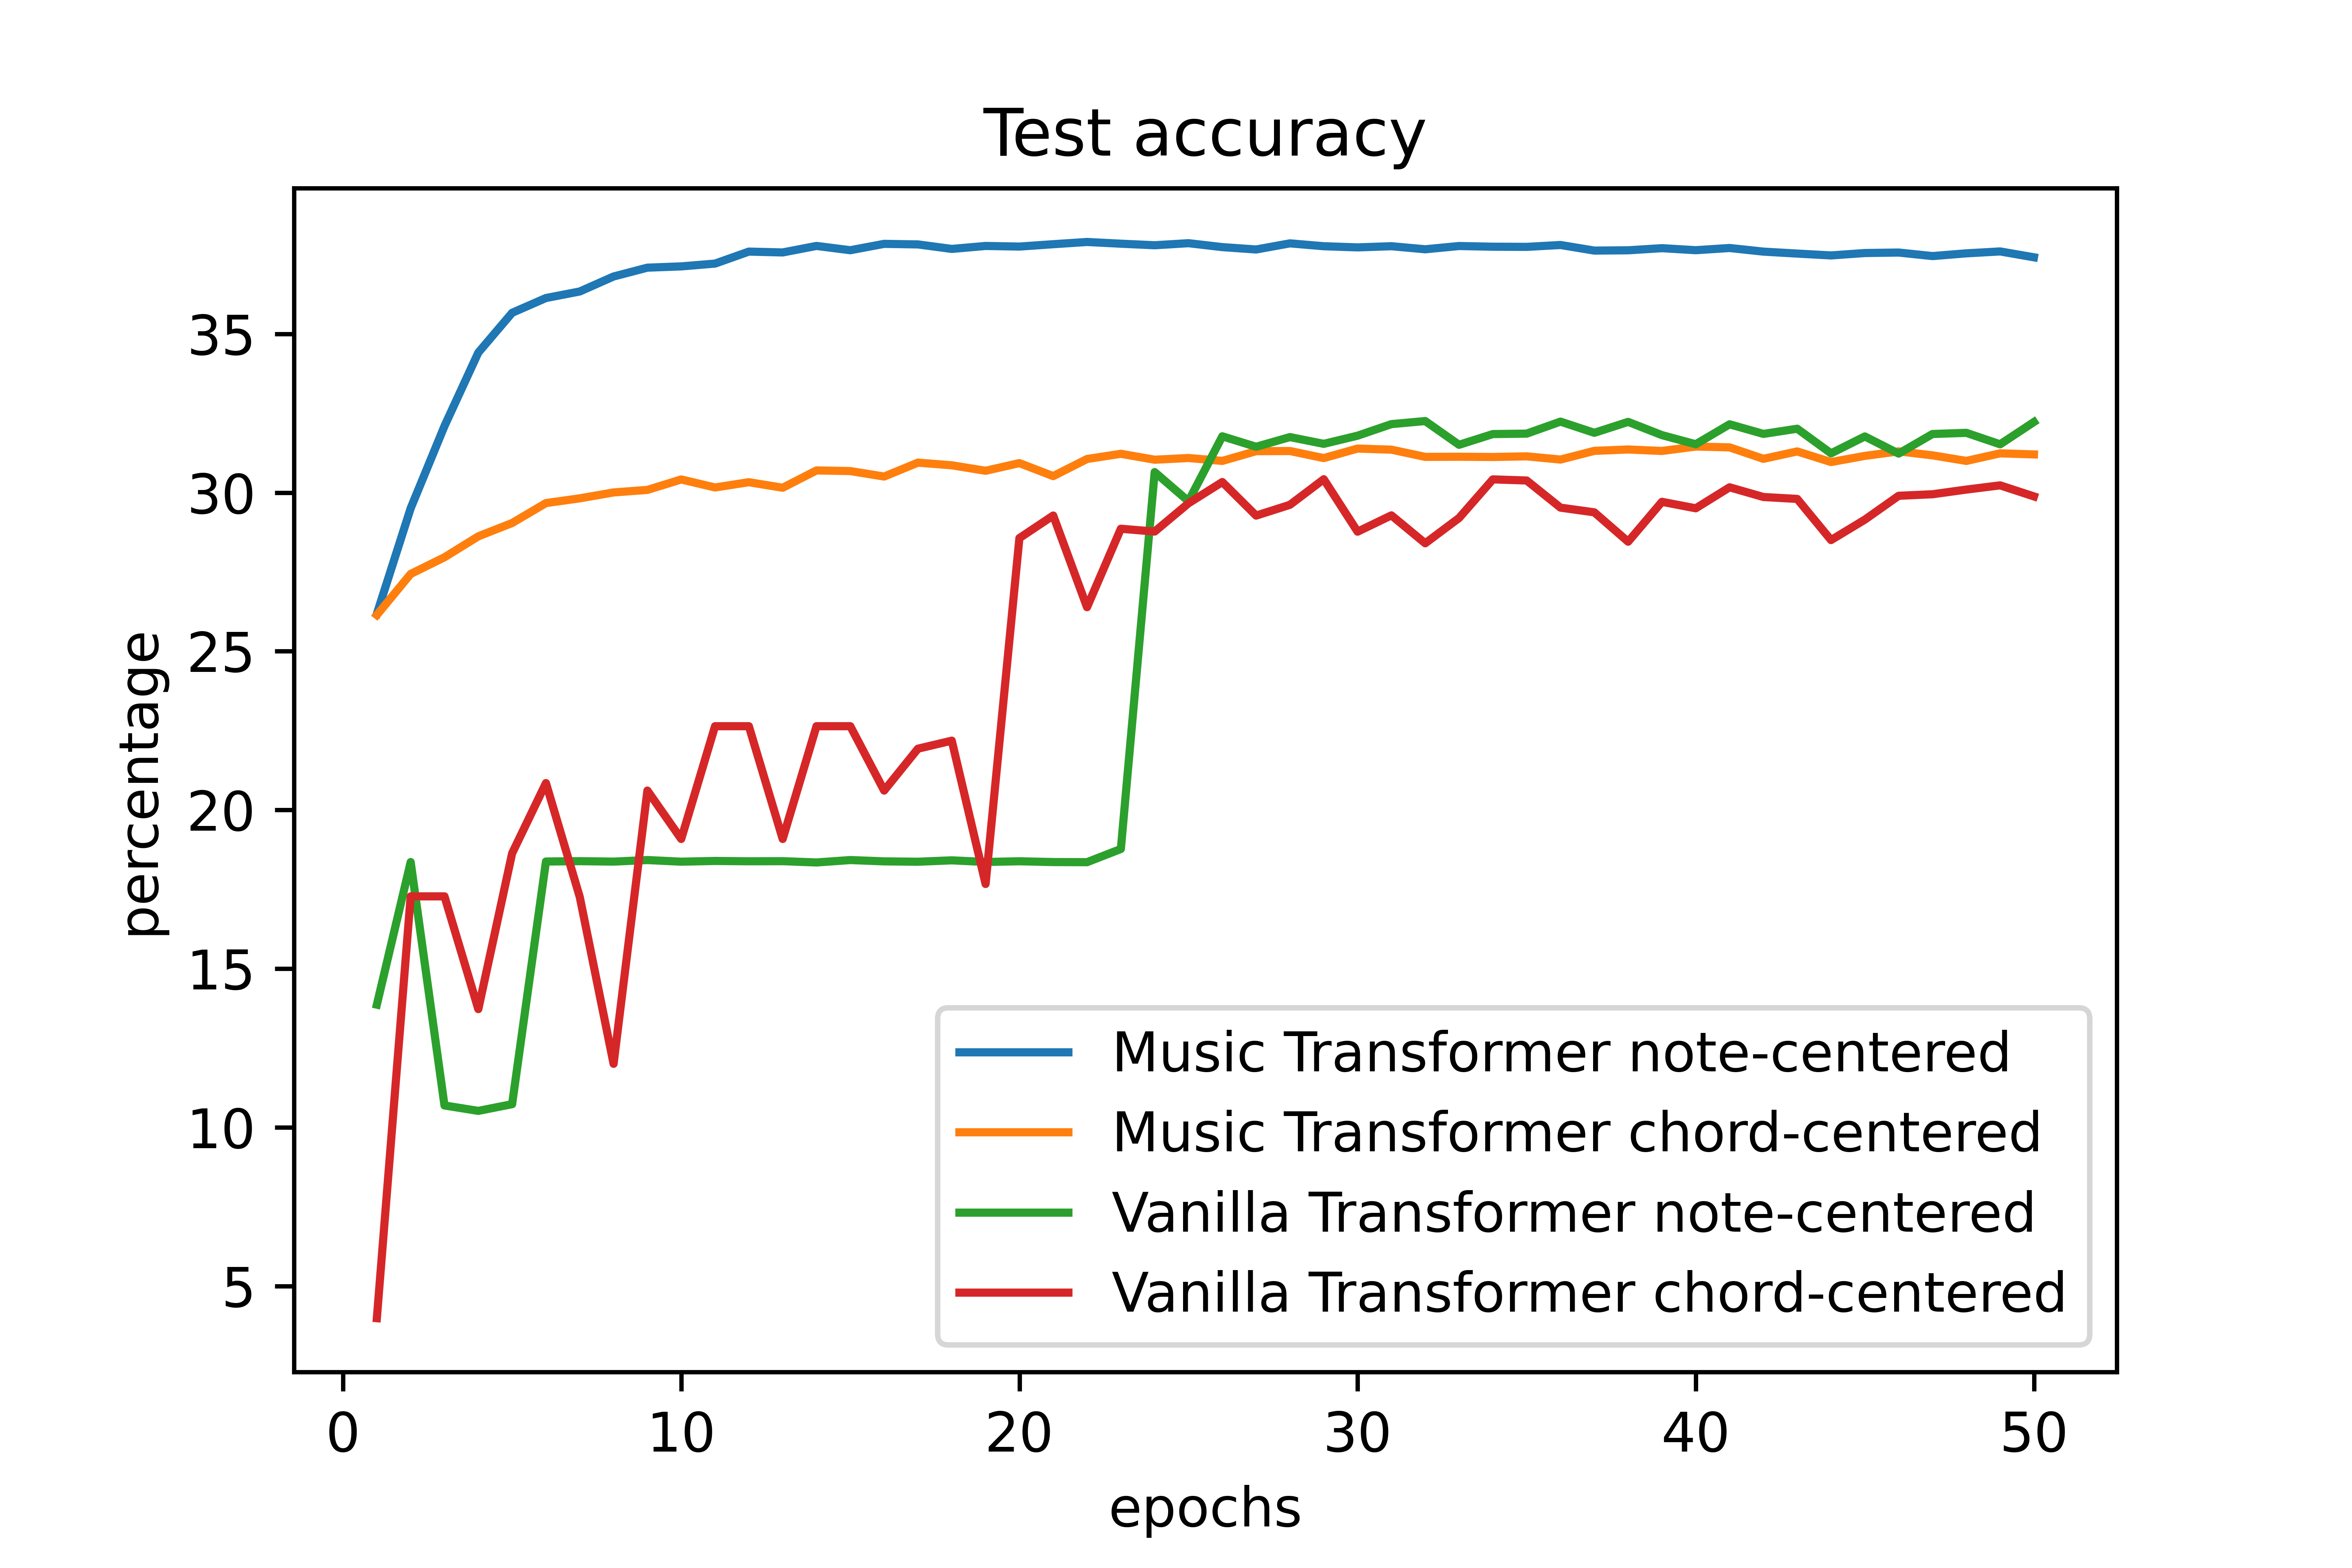
\includegraphics[width=0.8\textwidth]{assets/test-accuracy}
    \caption{~Accuracy of models on test set}\label{fig:test-accuracy}
\end{figure}

\begin{figure}
    \centering
    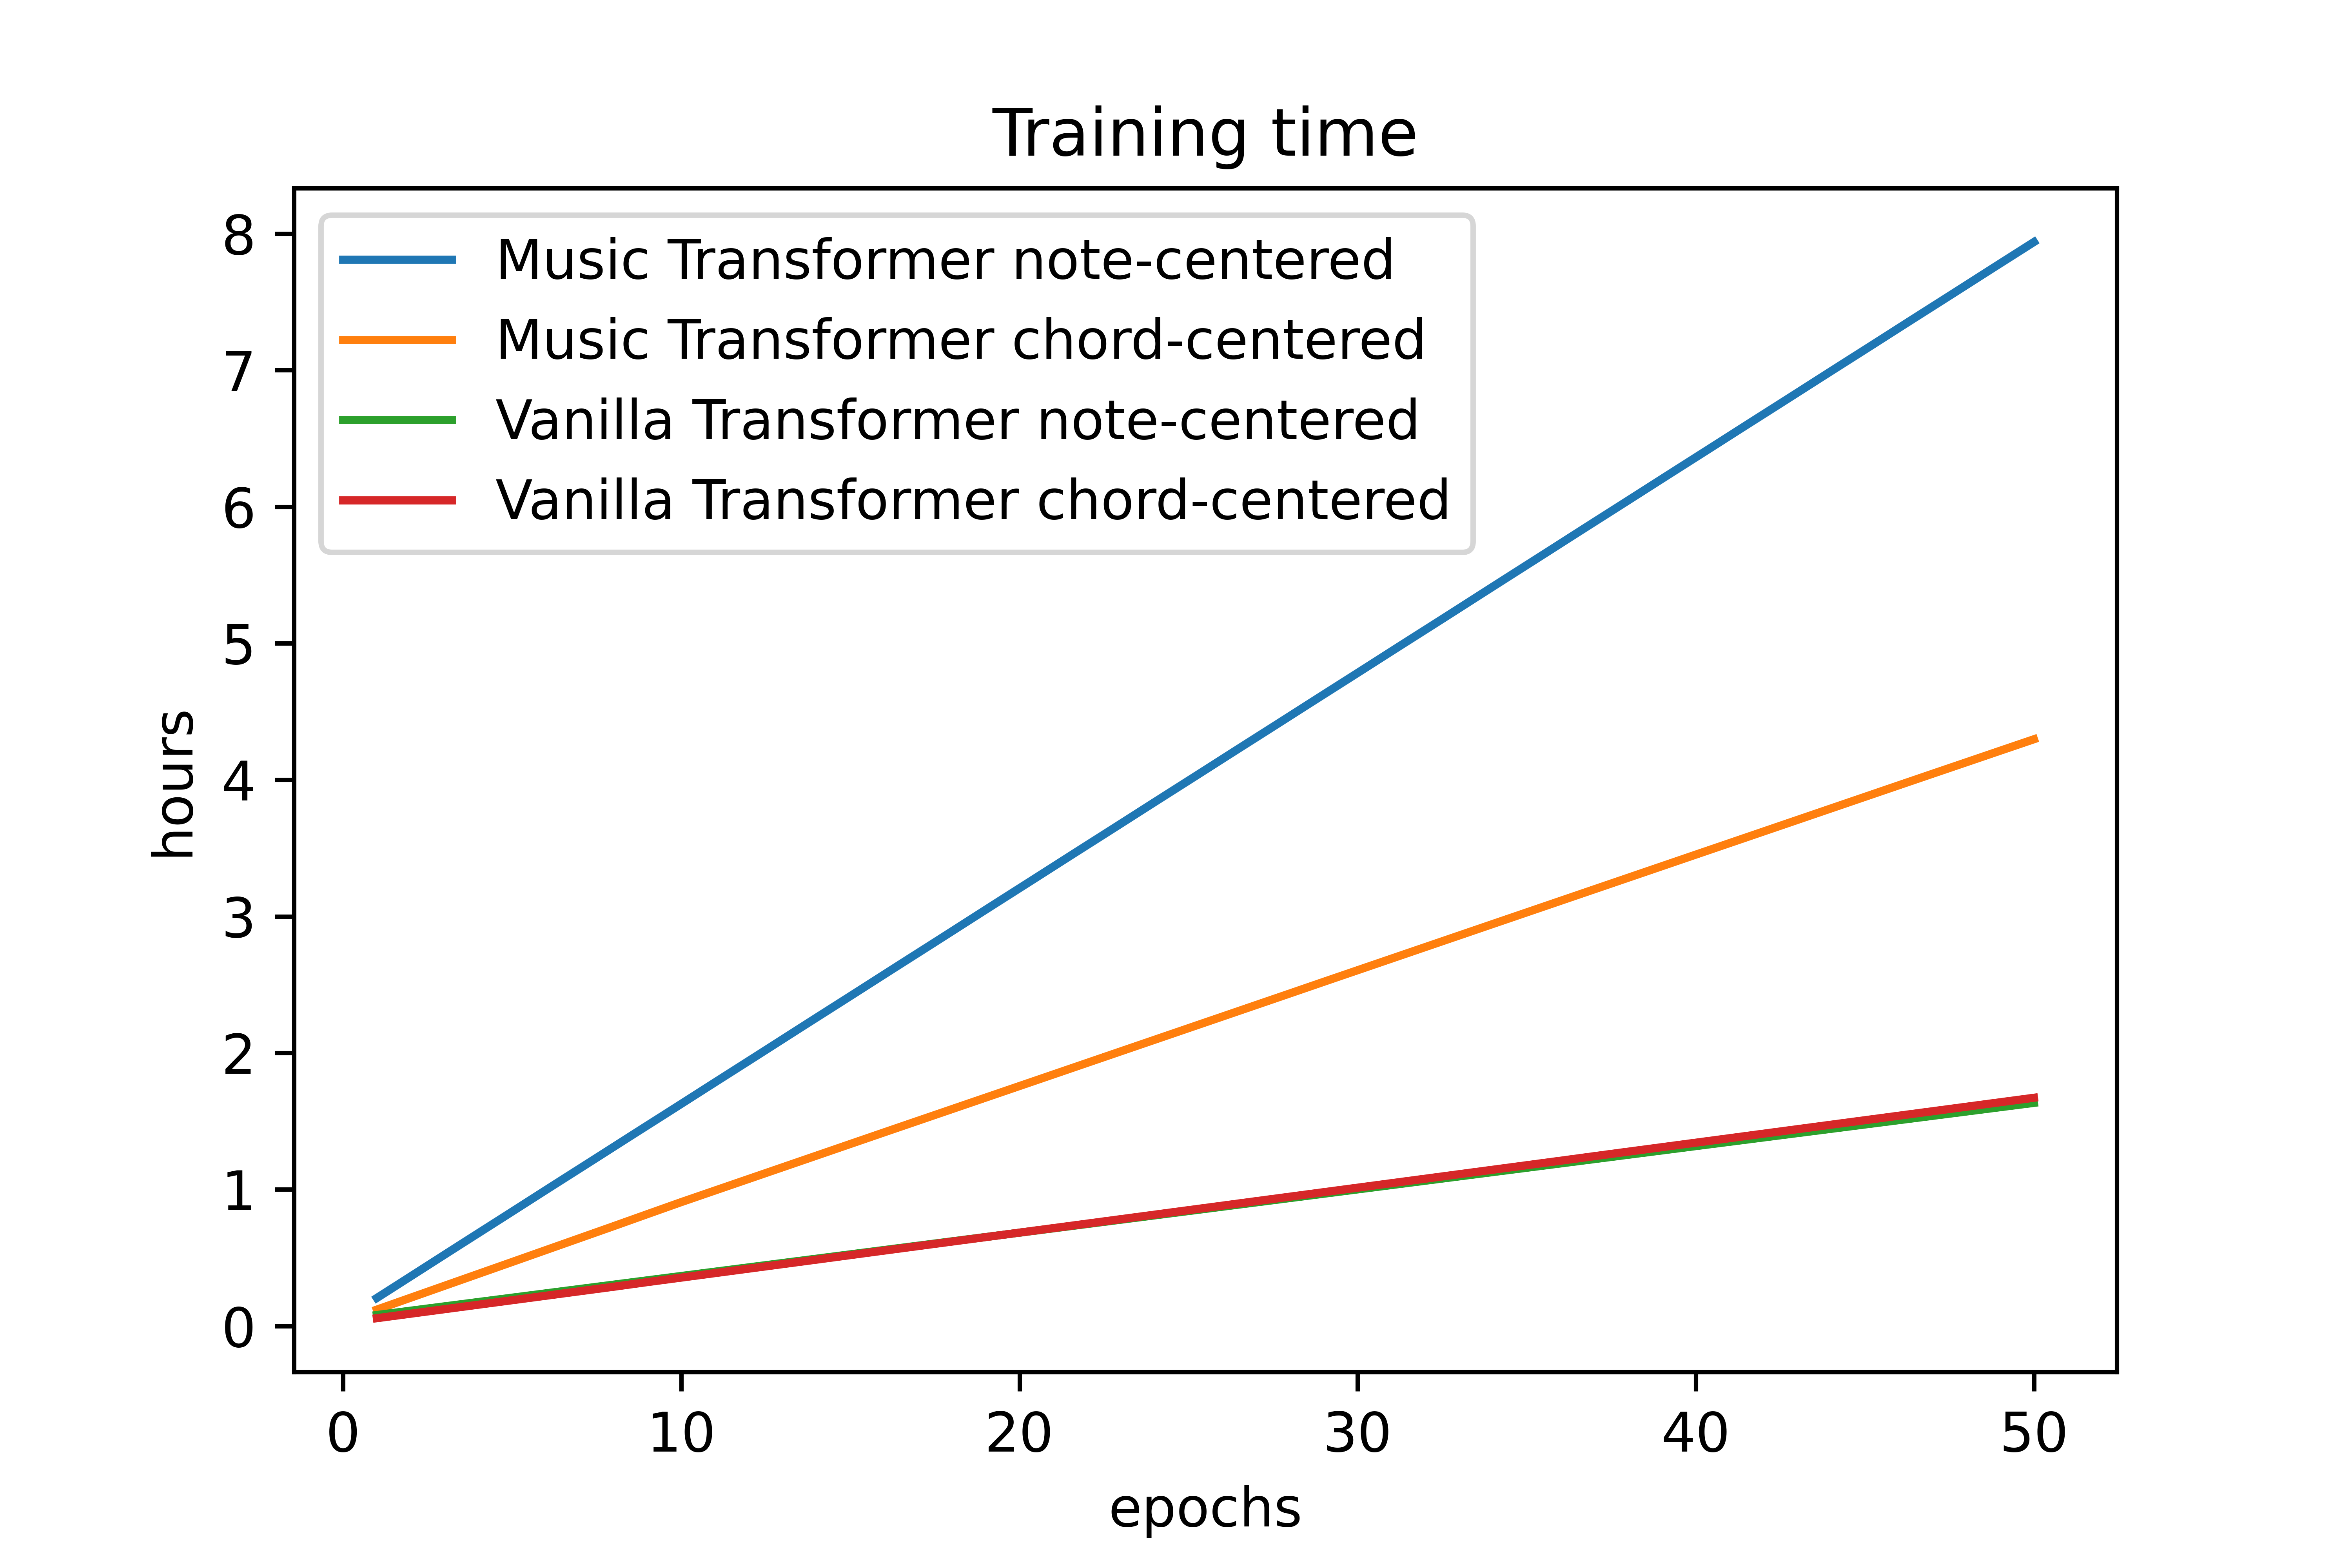
\includegraphics[width=0.8\textwidth]{assets/training-time}
    \caption{~Models training time}\label{fig:training-time}
\end{figure}

On the other hand, this is fixed with the Music Transformer, where the model always generates a non-empty composition.
Instead, it has the opposite problem.
When listening to the generated compositions, it can be heard that there are too many notes being played simultaneously, which does not sound very pleasant.
This problem is more significant for the chord-centered tokenization than the note-centered tokenization.
We provide a table with validation results for all of the models.

\begin{center}
    \begin{tabular}{|l|r|r|r|}
        \hline
        \textbf{Model}      & \textbf{Tokenization} & \textbf{Validation accuracy} & \textbf{Validation loss} \\
        \hline
        Vanilla Transformer & note                  & 30.34 \%                     & 2.83                     \\
        \hline
        Vanilla Transformer & chord                 & 28.23 \%                     & 4.58                     \\
        \hline
        Music Transformer   & note                  & 21.60 \%                     & 3.74                     \\
        \hline
        Music Transformer   & chord                 & 25.13 \%                     & 5.77                     \\
        \hline
    \end{tabular}
\end{center}